\documentclass[tikz,border=5pt]{standalone}
\usepackage{tikz}
\usetikzlibrary{shapes.geometric, arrows.meta, positioning, shadows}

\begin{document}
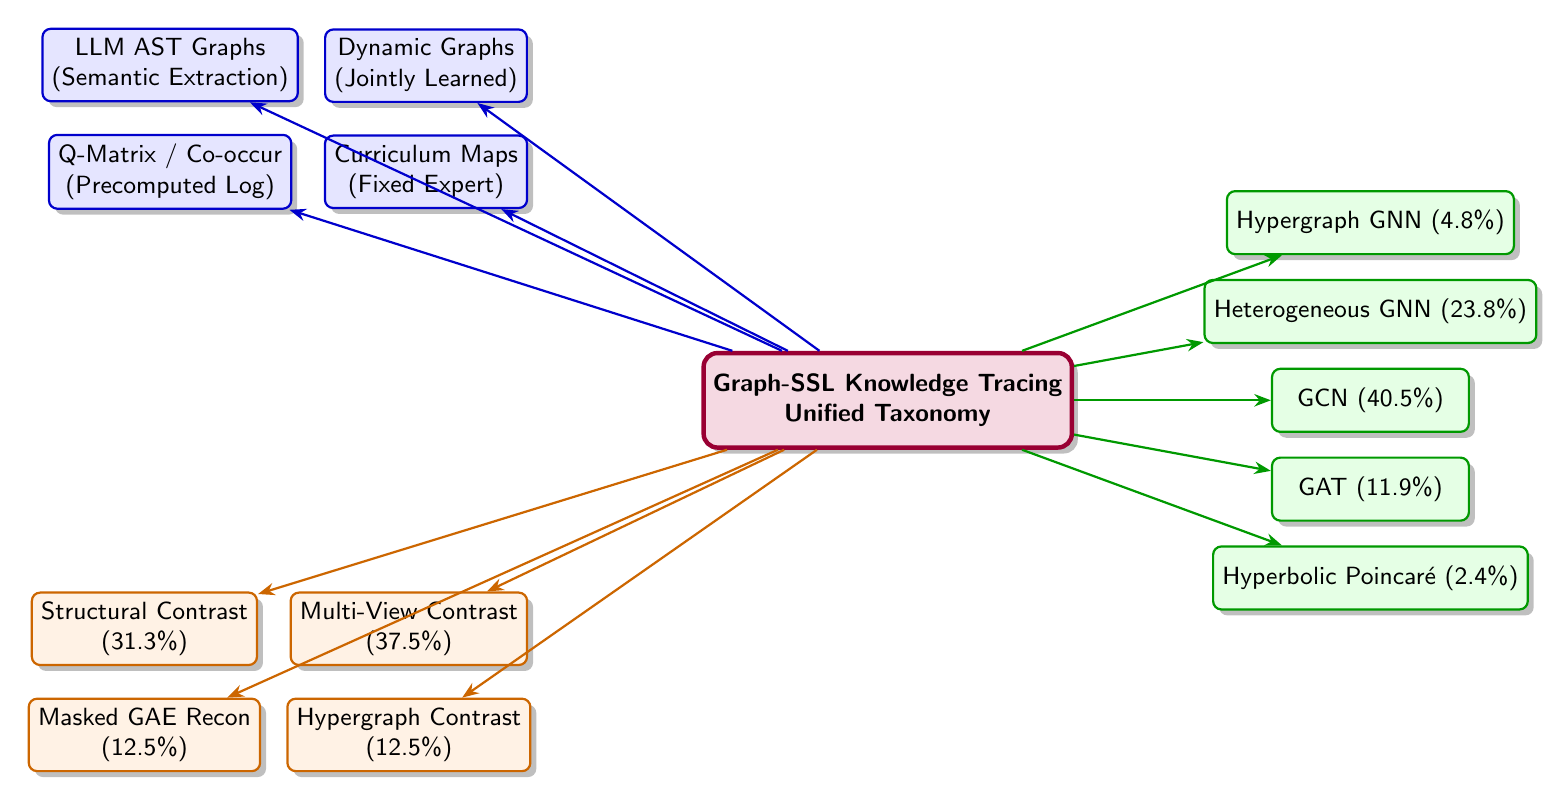
\begin{tikzpicture}[
    node distance=1.2cm and 1.5cm,
    font=\sffamily\small,
    box/.style={rectangle, draw=blue!80!black, fill=blue!10, thick, rounded corners=3pt, align=center, minimum width=2.5cm, minimum height=0.8cm, drop shadow},
    gnnbox/.style={rectangle, draw=green!60!black, fill=green!10, thick, rounded corners=3pt, align=center, minimum width=2.5cm, minimum height=0.8cm, drop shadow},
    sslbox/.style={rectangle, draw=orange!80!black, fill=orange!10, thick, rounded corners=3pt, align=center, minimum width=2.5cm, minimum height=0.8cm, drop shadow},
    arrow/.style={-{Stealth[length=6pt]}, thick, draw=gray!80}
]

% Center Root
\node[rectangle, draw=purple!80!black, fill=purple!15, ultra thick, rounded corners=5pt, align=center, minimum width=3.5cm, minimum height=1.2cm, drop shadow] (root) {\textbf{Graph-SSL Knowledge Tracing}\\\textbf{Unified Taxonomy}};

% Branch 1: Graph Sources (Top Left)
\node[box, above left=1.8cm and 2.2cm of root] (g_curric) {Curriculum Maps\\(Fixed Expert)};
\node[box, left=0.4cm of g_curric] (g_qmatrix) {Q-Matrix / Co-occur\\(Precomputed Log)};
\node[box, above=0.4cm of g_curric] (g_dynamic) {Dynamic Graphs\\(Jointly Learned)};
\node[box, above=0.4cm of g_qmatrix] (g_llm) {LLM AST Graphs\\(Semantic Extraction)};

% Branch 2: GNN Encoders (Right)
\node[gnnbox, right=2.5cm of root] (gnn_gcn) {GCN (40.5\%)};
\node[gnnbox, above=0.3cm of gnn_gcn] (gnn_hetero) {Heterogeneous GNN (23.8\%)};
\node[gnnbox, below=0.3cm of gnn_gcn] (gnn_gat) {GAT (11.9\%)};
\node[gnnbox, above=0.3cm of gnn_hetero] (gnn_hyper) {Hypergraph GNN (4.8\%)};
\node[gnnbox, below=0.3cm of gnn_gat] (gnn_hyperbolic) {Hyperbolic Poincaré (2.4\%)};

% Branch 3: SSL Pretext Objectives (Bottom Left)
\node[sslbox, below left=1.8cm and 2.2cm of root] (ssl_multiview) {Multi-View Contrast\\(37.5\%)};
\node[sslbox, left=0.4cm of ssl_multiview] (ssl_struct) {Structural Contrast\\(31.3\%)};
\node[sslbox, below=0.4cm of ssl_multiview] (ssl_hyper) {Hypergraph Contrast\\(12.5\%)};
\node[sslbox, below=0.4cm of ssl_struct] (ssl_gae) {Masked GAE Recon\\(12.5\%)};

% Connections
\draw[arrow, blue!80!black] (root) -- (g_curric);
\draw[arrow, blue!80!black] (root) -- (g_qmatrix);
\draw[arrow, blue!80!black] (root) -- (g_dynamic);
\draw[arrow, blue!80!black] (root) -- (g_llm);

\draw[arrow, green!60!black] (root) -- (gnn_gcn);
\draw[arrow, green!60!black] (root) -- (gnn_hetero);
\draw[arrow, green!60!black] (root) -- (gnn_gat);
\draw[arrow, green!60!black] (root) -- (gnn_hyper);
\draw[arrow, green!60!black] (root) -- (gnn_hyperbolic);

\draw[arrow, orange!80!black] (root) -- (ssl_multiview);
\draw[arrow, orange!80!black] (root) -- (ssl_struct);
\draw[arrow, orange!80!black] (root) -- (ssl_hyper);
\draw[arrow, orange!80!black] (root) -- (ssl_gae);

\end{tikzpicture}
\end{document}
